\documentclass{article}
\usepackage[UTF8]{ctex}
% Replace `letterpaper' with`a4paper' for UK/EU standard size
\usepackage[a4paper,top=2cm,bottom=2cm,left=3cm,right=3cm,marginparwidth=1.75cm]{geometry}

% Useful packages
\usepackage{amsmath}
\usepackage{cases}
\usepackage{mathrsfs,amsmath}
\usepackage{graphicx}
\usepackage[colorlinks=true, allcolors=blue]{hyperref}
\usepackage{graphicx} %插入图片的宏包
\usepackage{float} %设置图片浮动位置的宏包
\usepackage{subfigure} %插入多图时用子图显示的宏包
\usepackage{parskip}
\usepackage{indentfirst} 
\setlength{\parindent}{2em}
\usepackage{hyperref}  
\usepackage{tikz}
\allowdisplaybreaks
\usepackage{multirow}
\usepackage{amsmath}
\usepackage{amsfonts,amssymb} 
\usepackage{xcolor} % 用于显示颜色
\usepackage{listings} % 用于插入代码
\lstset{
	basicstyle          =   \sffamily,          % 基本代码风格
	keywordstyle        =   \bfseries,          % 关键字风格
	commentstyle        =   \rmfamily\itshape,  % 注释的风格,斜体
	stringstyle         =   \ttfamily,  % 字符串风格
	flexiblecolumns,                % 别问为什么,加上这个
	numbers             =   left,   % 行号的位置在左边
	showspaces          =   false,  % 是否显示空格,显示了有点乱,所以不现实了
	numberstyle         =   \zihao{-5}\ttfamily,    % 行号的样式,小五号,tt等宽字体
	showstringspaces    =   false,
	captionpos          =   t,      % 这段代码的名字所呈现的位置,t指的是top上面
	frame               =   lrtb,   % 显示边框
}

\lstdefinestyle{Python}{
	language        =   Python, % 语言选Python
	basicstyle      =   \zihao{-5}\ttfamily,
	numberstyle     =   \zihao{-5}\ttfamily,
	keywordstyle    =   \color{blue},
	keywordstyle    =   [2] \color{teal},
	stringstyle     =   \color{magenta},
	commentstyle    =   \color{red}\ttfamily,
	breaklines      =   true,   % 自动换行,建议不要写太长的行
	columns         =   fixed,  % 如果不加这一句,字间距就不固定,很丑,必须加
	basewidth       =   0.5em,
}

\title{图像处理与可视化 Homework-8 报告}
\author{林子开 21307110161}
\begin{document}
	\maketitle
	\tableofcontents

\section{在VTK中实现面绘制和体绘制}
在VTK中进行数据可视化的流程如b下:
\[
\text{Source/Reader} \rightarrow \text{Filter} \rightarrow \text{Mapper} \rightarrow \text{Actor}
\rightarrow \text{Renderer} \rightarrow \text{Render Window} \rightarrow \text{Interactor}    
\]

在本次试验中,统一使用老师提供的$\text{image\_lr.nii.gz}$数据。

\subsection{面绘制}
面绘制的Python代码如下:
\lstinputlisting[style = Python,
caption={面绘制的Python代码},
label = {面绘制}]{面绘制.py} 

面绘制的效果如下:
\begin{figure}[H]
	\centering
	{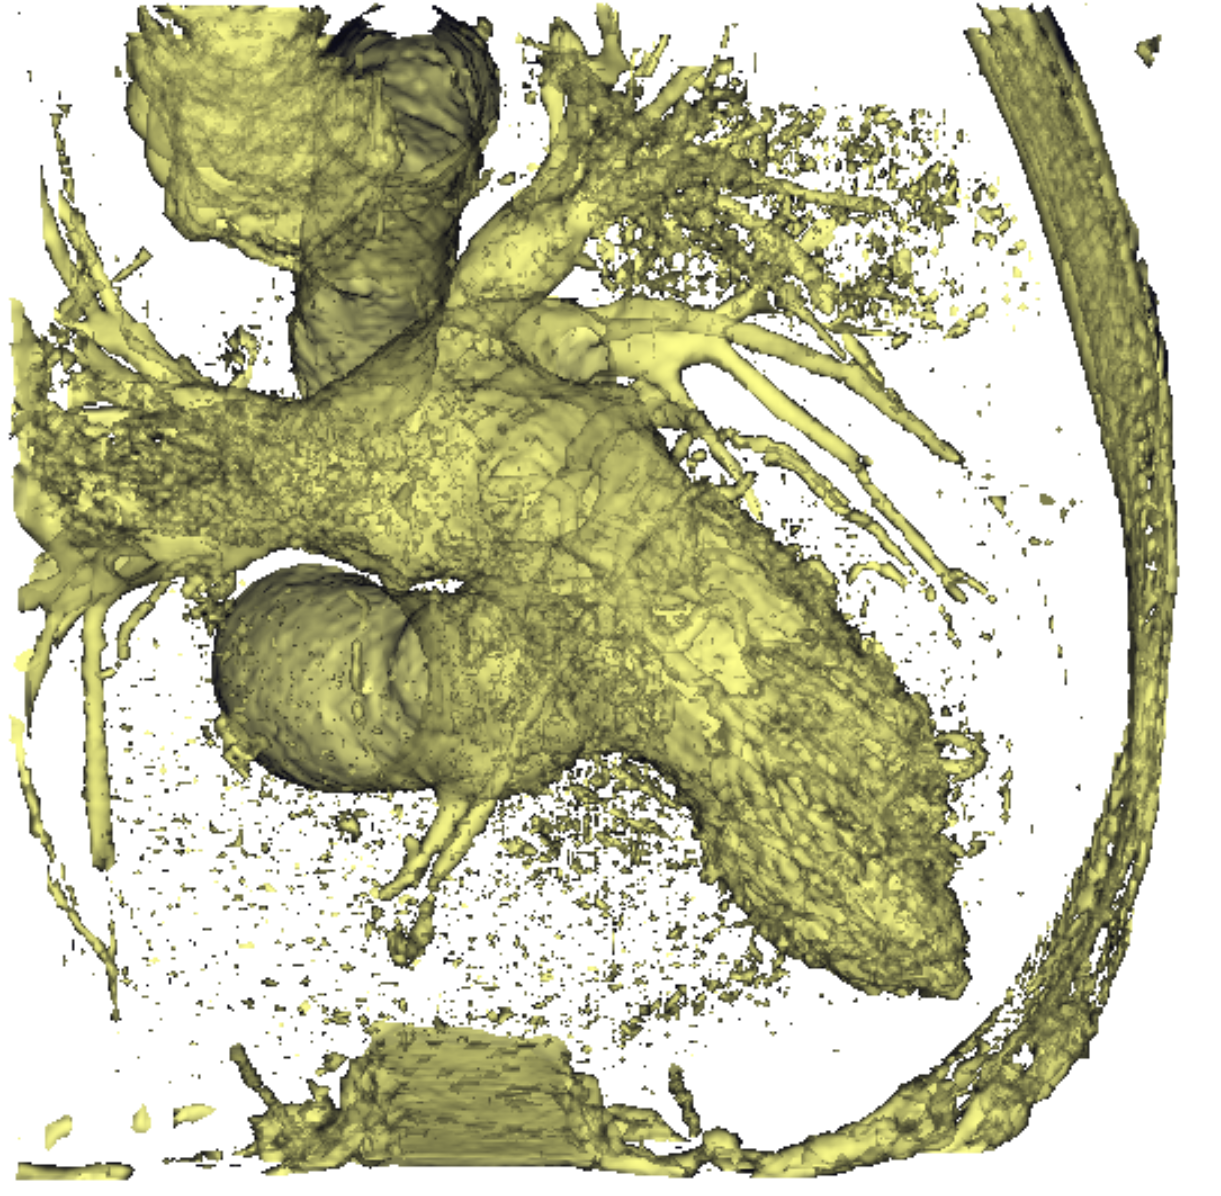
\includegraphics[width=0.5\textwidth]{image//面绘制.png}} 
	\caption{面绘制效果} 
\end{figure}
可以看出,图中有很多碎片。

\subsection{体绘制}
体绘制的Python代码如下:
\lstinputlisting[style = Python,
caption={体绘制的Python代码},
label = {体绘制}]{体绘制.py} 
体绘制的效果如下:
\begin{figure}[H]
	\centering
	{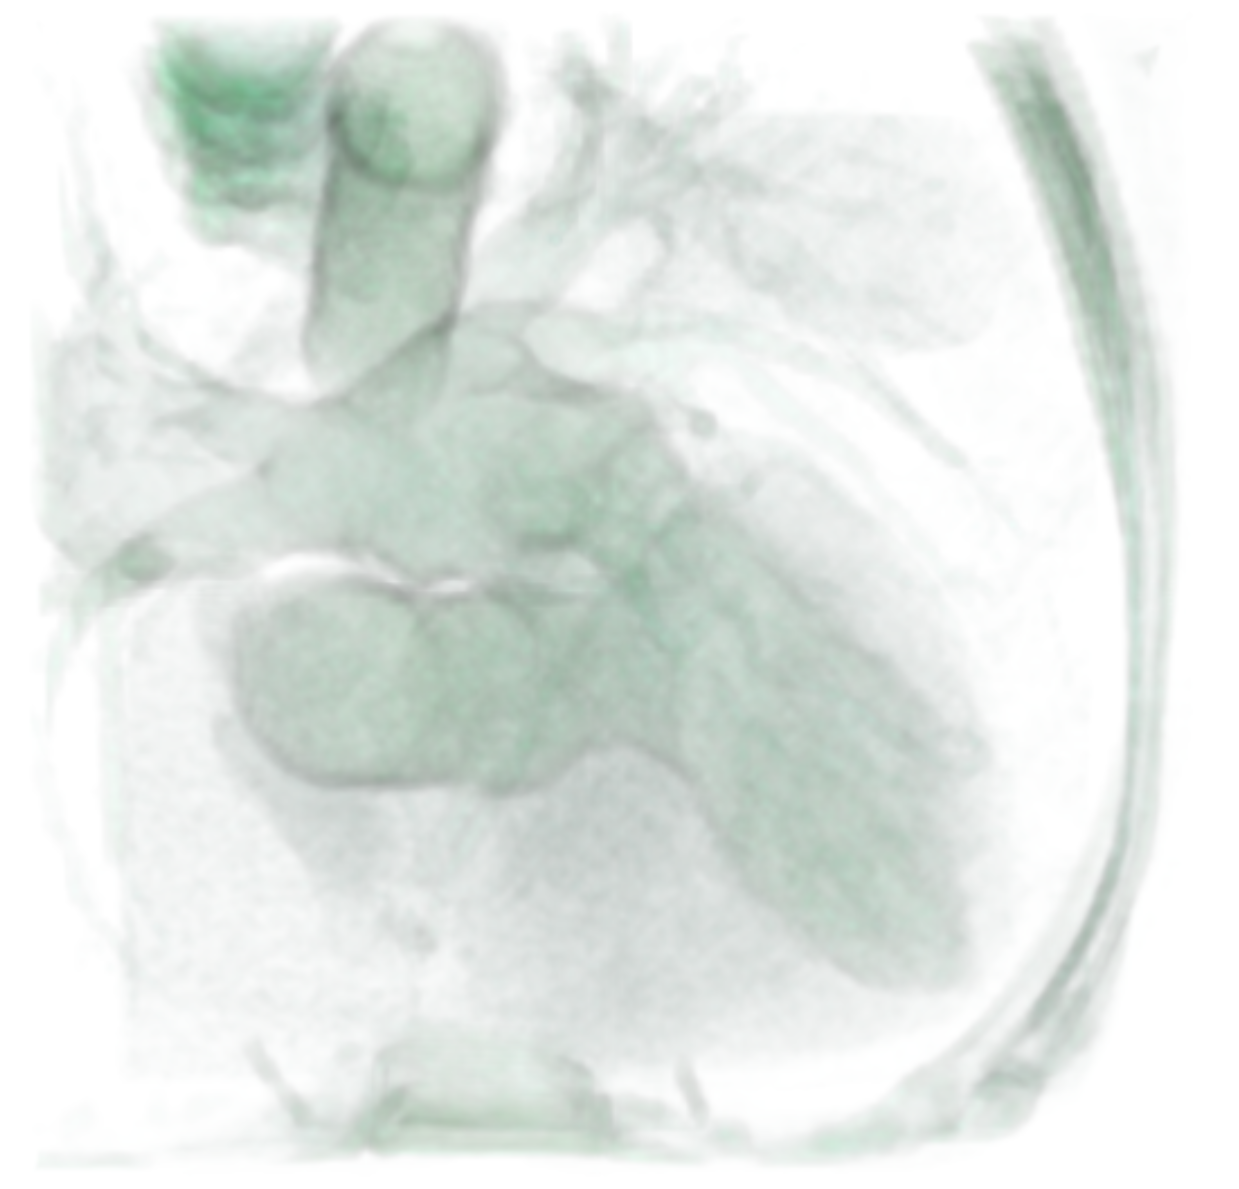
\includegraphics[width=0.5\textwidth]{image//体绘制.png}} 
	\caption{体绘制效果} 
\end{figure}

\section{消除碎片}
使用\texttt{vtk.vtkSmoothPolyDataFilter()}可以非常方便地消除碎片。
消除碎片的Python代码如下:
\lstinputlisting[style = Python,
caption={消除碎片的Python代码},
label = {消除碎片}]{消除碎片.py} 

消除碎片前后的效果对比图如下:
\begin{figure}[H]
    \centering
    \subfigure[消除碎片前]
    {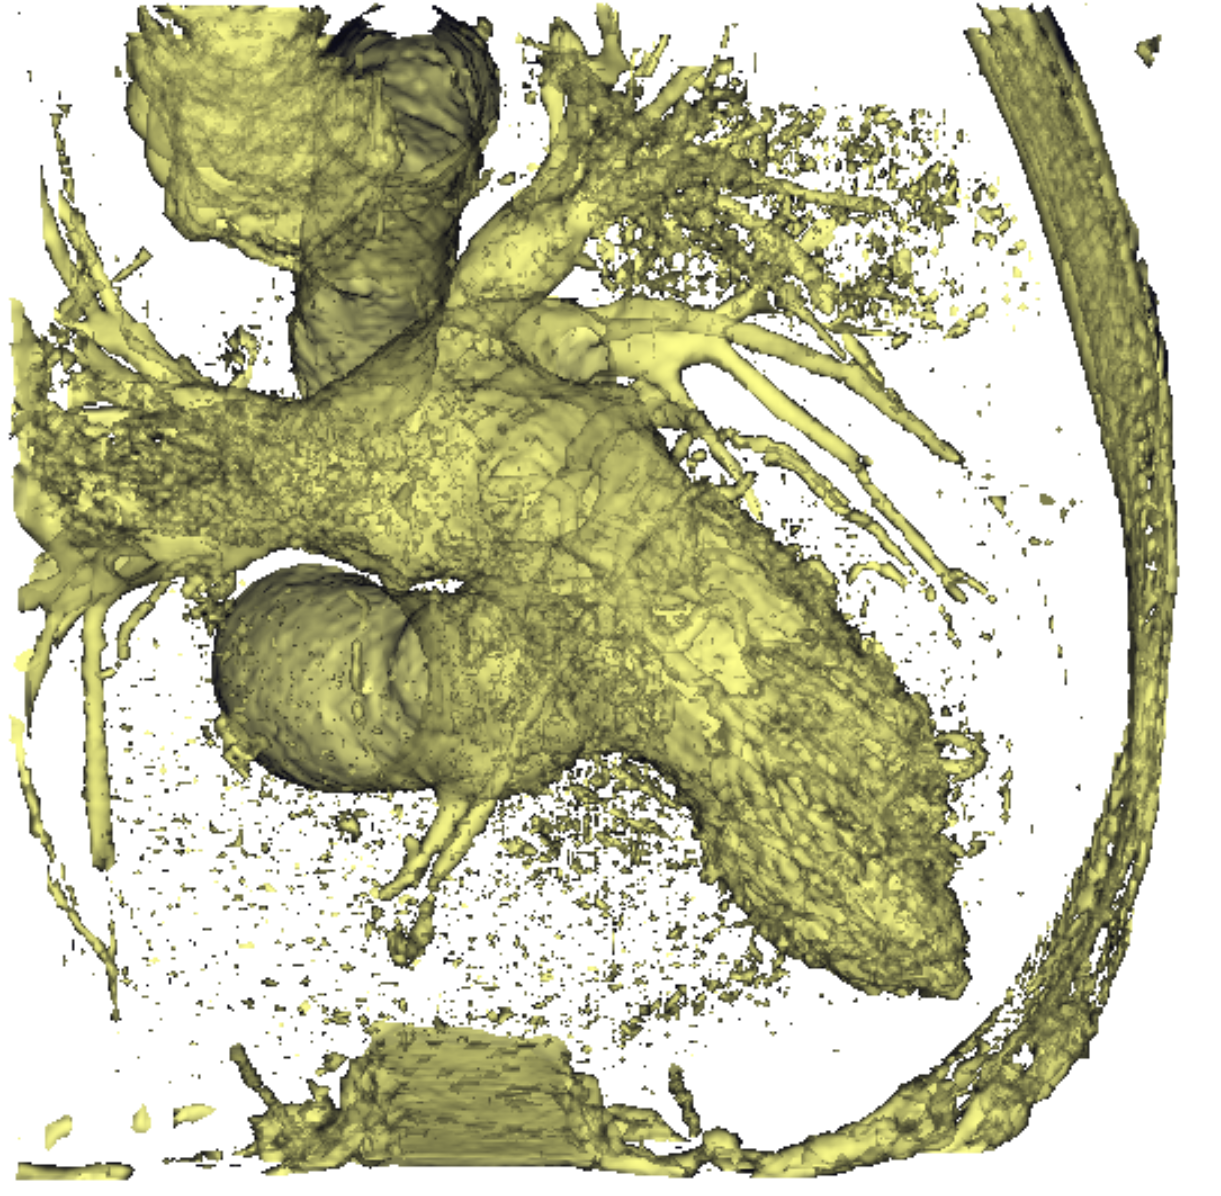
\includegraphics[width=0.45\textwidth]{image//面绘制.png}}
    \,    
    \subfigure[消除碎片后]
    {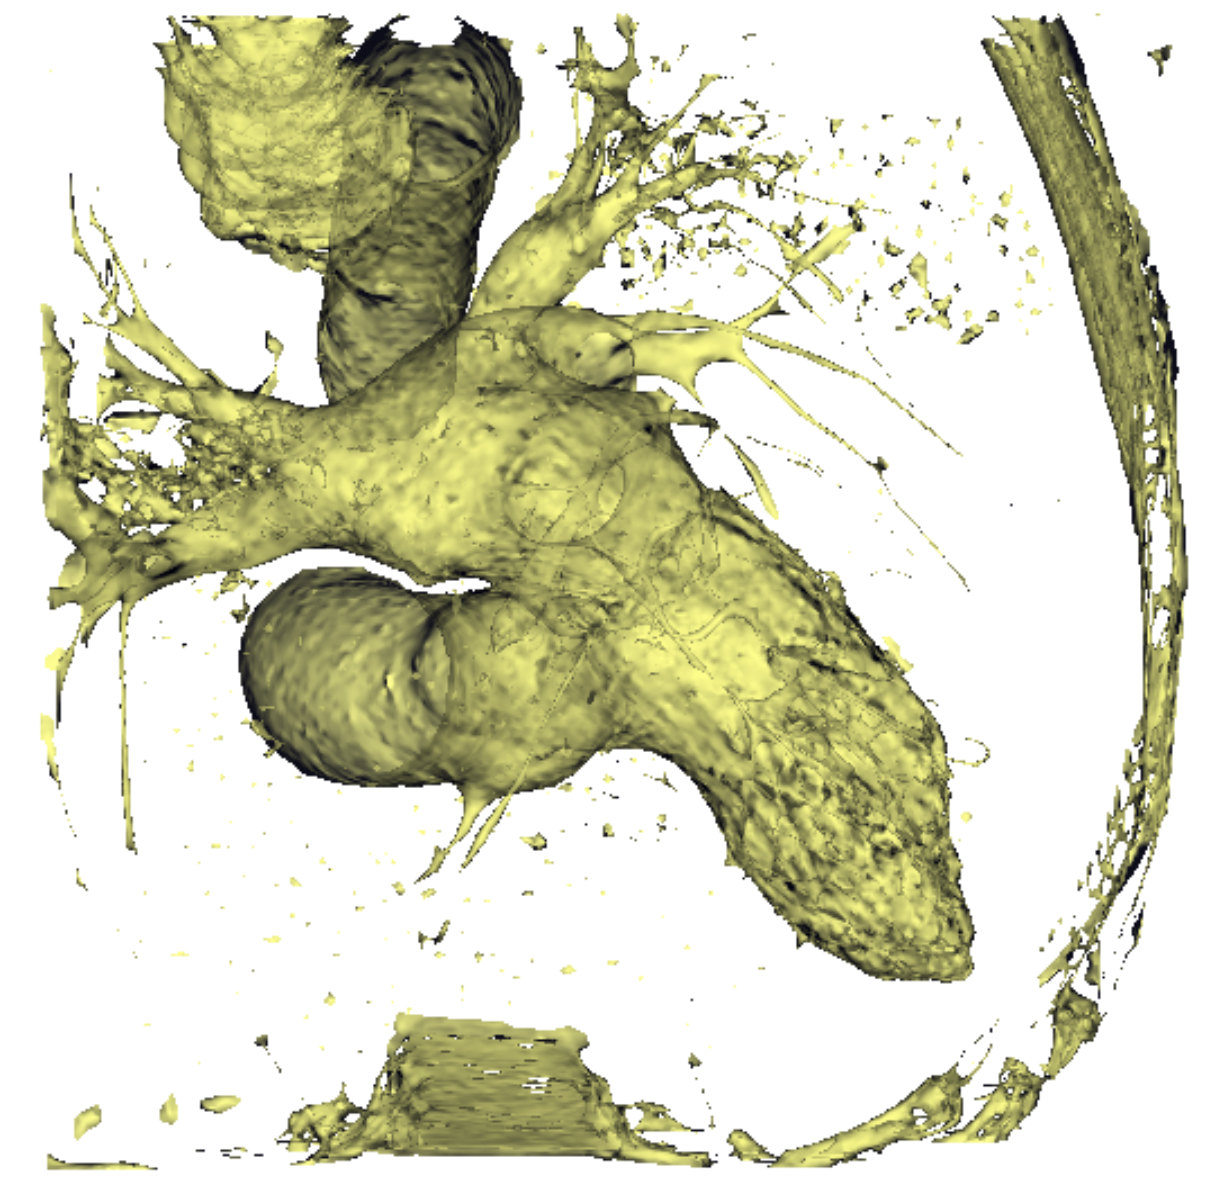
\includegraphics[width=0.45\textwidth]{image//消除碎片.png}}
    

\end{figure}


\end{document}

% \begin{figure}[H]
% 	\centering
% 	{\includegraphics[width=0.35\textwidth]{image//ignorance.png}} 
% 	\caption{} \label{} 
% \end{figure}


% \lstinputlisting[style = Python,
% caption={Python codes},
% label = {efficient},
% linerange={110-125}]{exercise3.py} 


% \begin{figure}[H]
%     \centering
%     \subfigure[patch size = 11]
%     {\label{} 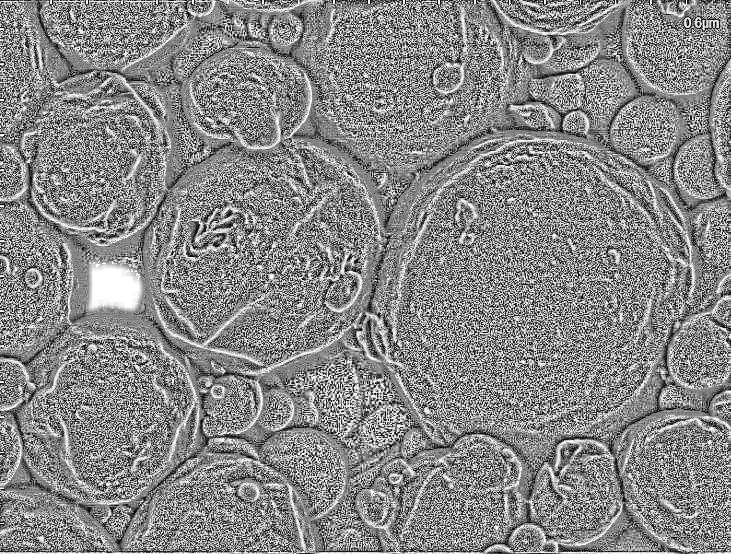
\includegraphics[width=0.49\textwidth]{image//local equalization with patch size = 11.jpg}}
%     \,    
%     \subfigure[patch size = 51]
%     {\label{} 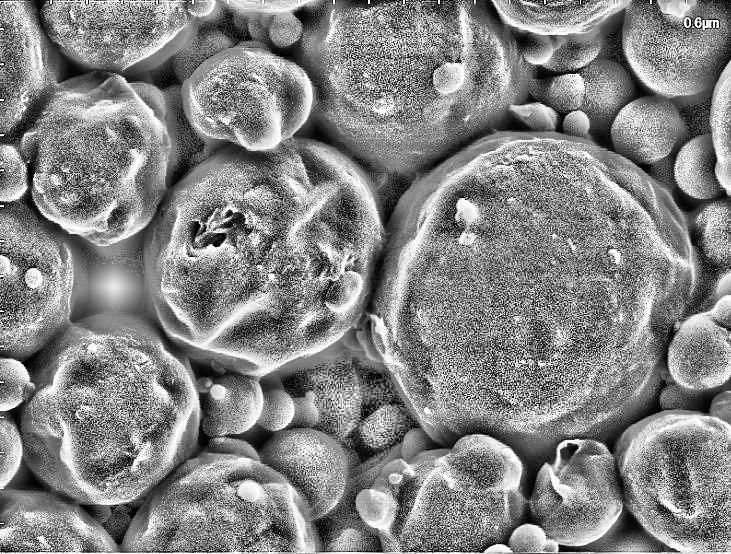
\includegraphics[width=0.49\textwidth]{image//local equalization with patch size = 51.jpg}}
%     \,
%     \subfigure[patch size = 151]
%     {\label{} 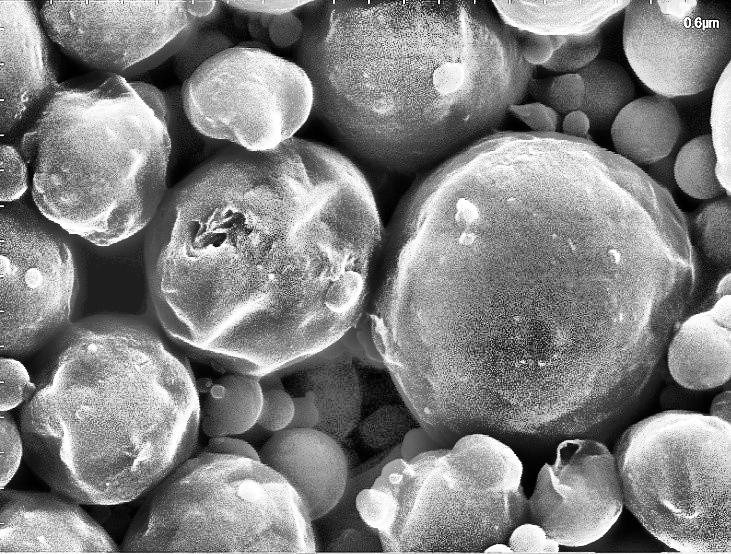
\includegraphics[width=0.49\textwidth]{image//local equalization with patch size = 151.jpg}}
%     \,    
%     \subfigure[patch size = 201]
%     {\label{} 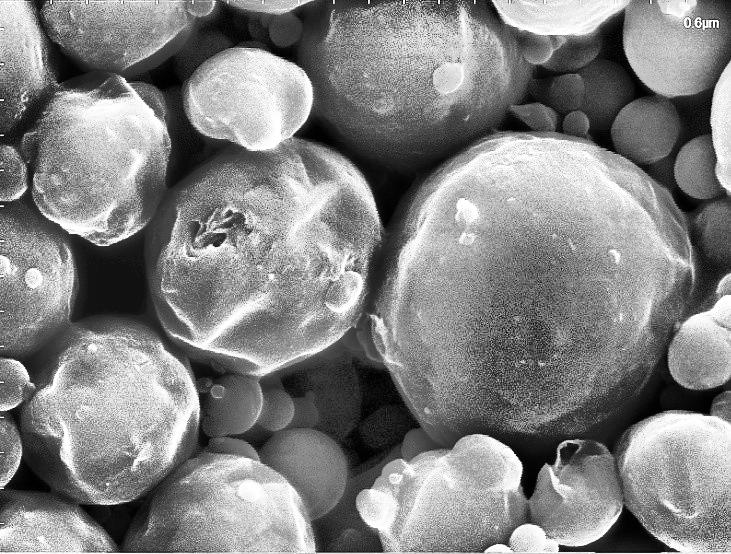
\includegraphics[width=0.49\textwidth]{image//local equalization with patch size = 201.jpg}}
%     \caption{local equalization with different patch sizes}\label{} 
% \end{figure}

% 矩阵$\Pi$的更新过程为:
% \begin{equation}

% 	\pi_{ij}^{(k)} = 
% 	\begin{cases}
% 		\pi_{ij}^{(k-1)} & \text{if $d_{ij}^{(k-1)}\le d_{ik}^{(k-1)} + d_{kj}^{(k-1)}$} \\
% 		\pi_{kj}^{(k-1)} & \text{if $d_{ij}^{(k-1)} > d_{ik}^{(k-1)} + d_{kj}^{(k-1)}$} 
% 	\end{cases}

% \end{equation}
